\chapter{Desenvolvimento de um rastreador de olhar usando CS}

\newc{Alguns algoritmos de rastreamento de olhar usam técnicas de processamento de imagens para identificar a posição da pupila. Essa tarefa é dificultada pela oclusão parcial da pupila pelos cílios. Em vez de estimar a posição da pupila, podemos comparar a imagem com amostras de imagens do olho onde a posição do olhar é conhecida e depois estimar o olhar a partir das posições de olhar das amostras mais parecidas com a imagem atual.

Usamos o modelo \textit{cross-and-bouquet} para comparar imagens das amostras e estimar a posição do olhar.}

Desenvolvemos um programa para estimar o olhar do usuário, ou seja, estimar qual coordenada $(x,y)$ na tela o usuário está olhando. Para isso, usamos câmera da Pupil Labs para coletar imagens do olho direito. Essa câmera fica acoplada à cabeça e registra imagens em infravermelho \footnote{\url{https://github.com/pupil-labs/pupil/wiki/Environment}}. O programa é dividido em duas etapas principais:

\begin{itemize}
\item {\bf Calibração:} exibimos alvos em posições específicas na tela e coletamos uma imagem do olho por alvo, assumindo que o usuário está olhando para o alvo.

\item {\bf Rastreamento:} para cada frame $f$, encontramos as amostras mais parecidas com $f$. Estimamos a posição do olhar como a média das posições da na tela correspondentes às amostras selecionadas.
\end{itemize}

Essas etapas são descritas mais detalhadamente abaixo.

\section{Coleta de amostras}

%Nesta etapa, o programa coleta uma imagem do olho correspondendo a cada uma das coordenadas na tela de uma grade com $10 \times 10$ pontos. Para cada alvo, é necessário que o usuário pressione uma tecla quando estiver olhando para o alvo para ler a amostra, como mostra a Figura \ref{fig:alvo}. Assumimos que o usuário não move a cabeça durante a coleta.

Fizemos o experimento com seis pessoas para avaliar o desempenho do rastreador de olhar. Durante o experimento o participante ficou sentado a $56,5cm$ de distância do monitor, com o olho direito alinhado com o centro da tela. Para evitar movimentos da cabeça durante a coleta das imagens, a pessoa ficou com o queixo apoiado sobre o punho e cotovelo correspondente apoiado na mesa. Registramos imagens do olho direito usando uma câmera do Pupil Labs, acoplada à cabeça, que grava imagens em infravermelho.

A câmera do Pupil Labs estava ligada a um suporte de formato parecido com uma armação de óculos. Por esse motivo, quem usa óculos teve que retirar os óculos para participar do experimento.

Antes de iniciar a coleta, mostramos a imagem da câmera do olho para a pessoa ajustar a câmera de forma que o olho inteiro esteja visível na imagem, como mostra a Figura \ref{fig:ajustando_olho}.

\begin{figure}
\centering
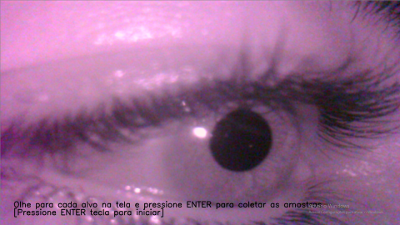
\includegraphics[scale=1]{imagens/ajustando_camera.png}
\caption{O programa exibe uma imagem do olho antes da coleta, para o usuário ajustar a câmera de forma que o olho inteiro seja registrado.}
\label{fig:ajustando_olho}
\end{figure}

Foram exibidos aleatoriamente $49$ pontos dispostos numa grade $7 \times 7$ de pontos igualmente espaçados, onde a distância entre cada lado da grade e o canto correspondente da tela corresponde a um grau do campo visual.

Mostramos cada alvo individualmente durante dois segundos e o usuário deveria olhar para o ponto, como mostra a Figura $\ref{fig:alvo}$. Mostramos os pontos aleatoriamente para evitar aprendizado do usuário, ou seja, evitar que o usuário olhe para o ponto correspondendo à amostra seguinte antes de terminar a coleta da amostra atual. Apesar de mostrar cada ponto durante dois segundos, coletamos imagens apenas após o primeiro segundo porque durante os primeiros instantes ocorre a sacada, ou seja, o movimento do olhar até a região de interesse, e queremos registrar apenas imagens correspondendo à fixação, ou seja, quando a pessoa está realmente olhando para o ponto.

%Coletamos um número grande (cerca de 25 amostras por usuário por posição da tela) de imagens porque queremos comparar o desempenho de programa usando diferentes números de amostras para calibrar o rastreador, como explicaremos adiante.
Usamos um monitor de lagura $37,3cm$ e altura de $32cm$, com resolução $1280 \times 1024$. A coleta durou menos de $10$ minutos por participante.

\begin{figure}
\centering
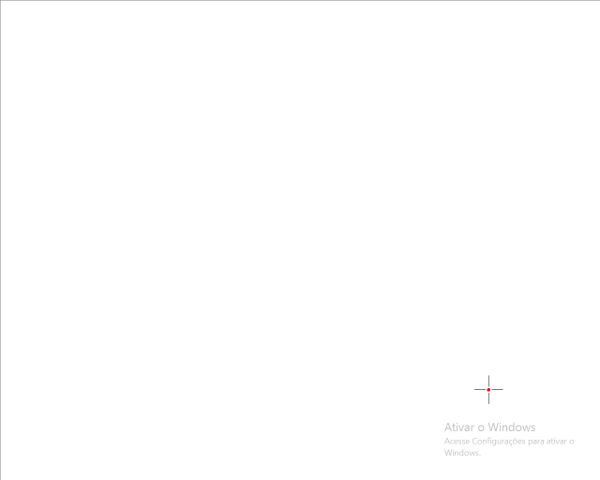
\includegraphics[scale=1]{imagens/alvo.png}
\caption{\oldc{Durante uma coleta, a pessoa deve olhar. Os alvos são exibidos em posições diferentes em uma grade $7 \times 7$ na tela.} \newc{Durante uma coleta, a pessoa deve olhar para os alvos que são exibidos em posições diferentes em uma grade $7 \times 7$.}}
\label{fig:alvo}
\end{figure}

\section{\newc{Rastreamento de olhar}}

Após terminar a coleta das imagens, estimamos a posição do olhar para imagens correspondendo a todos os pontos da grade $7 \times 7$. Como todas imagens registradas correspondem aos pontos da grade, já sabemos a posição do olhar em cada um deles, então usaremos a posição exata e a posição estimada para calcular o erro como a distância euclidiana entre elas. Usaremos a posição de cada alvo em graus horizontal e vertical, e não em \textit{pixels} na tela.

Para cada posição na grade, consideramos a primeira imagem coletada como a amostra correspondente àquela posição na tela, e estimaremos a posição do olhar para cinco das outras imagens, selecionadas aleatoriamente, comparando esta com todas as amostras\newc{, como mostra a Figura $\ref{fig:matriz_olho}$.}

\begin{figure}
$$ A = \left[ \hspace{2pt} \raisebox{-9pt}{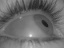
\includegraphics[scale=.6]{imagens/olhos/(0,0).jpg}} \hspace{2pt}\Bigg\vert\hspace{2pt} \raisebox{-9pt}{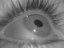
\includegraphics[scale=.6]{imagens/olhos/(2,4).jpg}}\hspace{2pt} \Bigg\vert\hspace{2pt} \raisebox{-9pt}{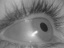
\includegraphics[scale=.6]{imagens/olhos/(4,1).jpg}} \hspace{2pt}\Bigg\vert \cdots \Bigg\vert \hspace{2pt}\raisebox{-9pt}{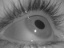
\includegraphics[scale=.6]{imagens/olhos/(6,4).jpg}}\hspace{2pt}  \right]$$

$$y = \left[ \hspace{2pt} \raisebox{-9pt}{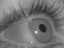
\includegraphics[scale=.6]{imagens/olhos/(5,2).jpg}} \hspace{2pt} \right]$$
\caption{Dada uma matriz com as amostras e uma imagem $y$, identificamos as amostras mais parecidas com $y$ usando o modelo \textit{cross-and-bouquet}, depois estimamos o olhar como a média ponderada das posições de olhar dessas amostras.}
\label{fig:matriz_olho}
\end{figure}

Pelo modelo \textit{cross-and-bouquet}, para cada vetor correspondendo à imagem $y$, calculamos um vetor $x = (c, e)$ tal que $y = Ac + e$. Podemos assumir que as amostras mais parecidas com $y$, são as colunas $a_i$ de $A$ onde $c_i$ possuem maior valor em módulo. Assumindo isso, estimamos a posição do olhar para a imagem $y$ como a média ponderada das posições do olhar das três imagens mais parecidas com $y$, onde $\vert c_i \vert$ são os pesos.

Antes de comparar as imagens usando o modelo \textit{cross-and-bouquet} reduzimos as imagens aplicando a pirâmide gaussiana $3$, $4$ ou $5$ vezes, resultando em imagens $60 \times 80$, $40 \times 30$ e $20 \times 15$, respectivamente. Fazemos isso para evitar erros de memória durante a execução do programa.

\newc{Após calcular a matriz $A$, estimamos o olhar de cada imagem. A entrada do algoritmo será então a imagem e a saída será a posição do olhar em graus do campo de visão do usuário.}

\section{Resultados}
A Tabela $\ref{tab:erros}$ mostra a média dos erros (conhecida como acurácia) e o desvio padrão (a precisão), considerando  diferentes tamanhos de imagens. Podemos observar que o erro é menor se usamos imagens maiores para estimar o olhar. Para imagens $60 \times 80$, obtemos uma acurácia de $1,053 $ e precisão de $2,279$, semelhantes aos resultados obtidos pelo rastreador Tobii EyeX, que tem acurácia de $1,42$ e precisão de $1,70$, segundo \cite{liboku}. \newc{A Tabela $\ref{tab:erros}$ indica também o tempo médio para estimar o olhar em cada imagem.}

\begin{table}
\centering
\begin{tabular}{| c | c | c | c |}
\hline
%& \multicolumn{3}{| c |}{dimensão das imagens} \\ \hline
dimensões das imagens & $15 \times 20$ & $30 \times 40$ & $60 \times 80$ \\ \hline
Erro				  & $1,471 \pm 2,398$ & $1,113 \pm 2,291$ & $1,053 \pm 2,279$ \\ \hline
Tempo de processamento & $0,035s$ & $0,215s$ & $5.311s$ \\ \hline
Imagem & \vspace{2pt} 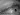
\includegraphics[width=2cm]{imagens/olho_20_15.jpg} & 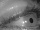
\includegraphics[width=2cm]{imagens/olho_40_30.jpg} & 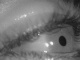
\includegraphics[width=2cm]{imagens/olho_80_60.jpg} \\ \hline
\end{tabular}
\caption{Erros na estimação do olhar para diferentes tamanhos de amostras. Cada coluna representa o tamanho das imagens usadas, e cada célula representa o erro médio $\pm$ o desvio padrão em graus. \newc{Vemos também o tempo médio para estimar o olhar de cada imagem.} A última linha mostra exemplos de imagens usadas nas respectivas dimensões.}
\label{tab:erros}
\end{table}

A Figura $\ref{fig:erros_posicao}$ mostra a distribuição dos erros nos pontos da grade para diferentes tamanhos de imagem, após reduzir as imagens originais aplicando a pirâmide gaussiana $3$ vezes (resultando em uma imagem $60 \times 80$, $4$ vezes (resultando em imagens $30 \times 40$ e $5$ vezes (resultando em imagens $15 \times 20$). Podemos notar na última imagem que os erros são maiores nos cantos da grade.

\begin{figure}
\centering
	\begin{subfigure}[b]{0.4\textwidth}
        \centering
        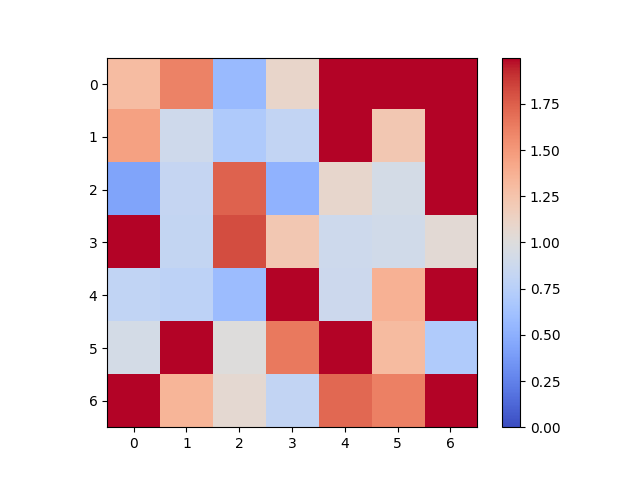
\includegraphics[scale=.4]{imagens/erros5pyrDown.png}
        \caption{}
    \end{subfigure}
    ~
    \begin{subfigure}[b]{0.4\textwidth}
        \centering
        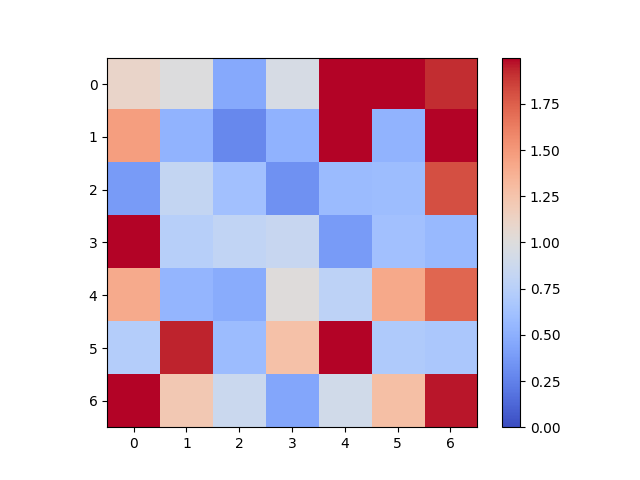
\includegraphics[scale=.4]{imagens/erros4pyrDown.png}
        \caption{}
    \end{subfigure}\\
    
    \begin{subfigure}[b]{0.4\textwidth}
        \centering
        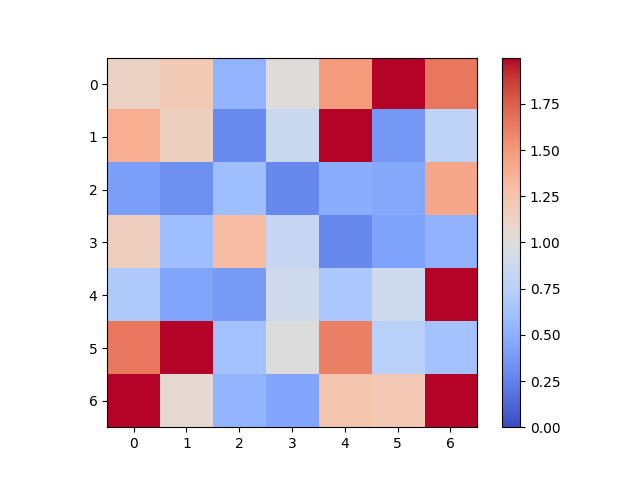
\includegraphics[scale=.4]{imagens/erros3pyrDown.png}
        \caption{}
    \end{subfigure}
        
    \caption{Erros médios para cada posição na grade, usando amostras correspondentes a uma grade $7 \times 7$. Em {\bf (a)} As imagens usadas têm dimensão $20 \times 15$, em {\bf (b)} as imagens são $40 \times 30$ e em {\bf (c)} as imagens são $60 \times 80$.}
    \label{fig:erros_posicao}
\end{figure}

A Figura \ref{fig:erros_participante} mostra a acurácia para cada participante. Observando os dados e as imagens registradas durante o experimento, notamos que se o participante piscar durante a coleta das amostras, o resultado será pior. O participante $2$, por exemplo, piscou algumas vezes durante a coleta de algumas amostras (que eram usadas para estimar o olhar nas outras imagens), acreditamos que por isso o resultado foi pior que os dos outros participantes.

\begin{figure}
    \centering
    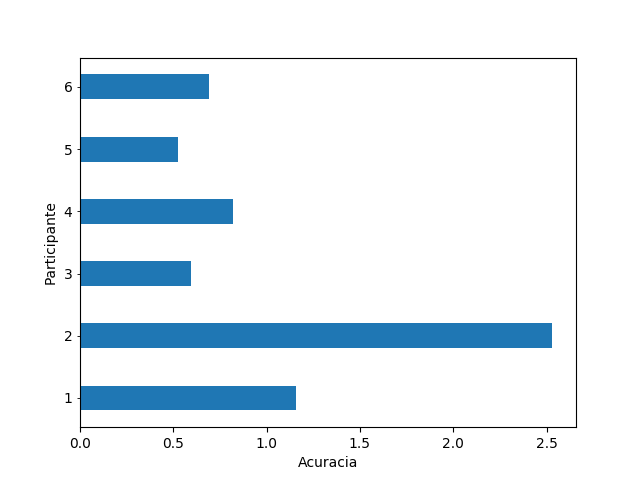
\includegraphics[scale=.6]{imagens/errosParticipantes_pyrDown3.png}
    \caption{A figura mostra a acurácia para diferentes participantes usando o algoritmo para estimar olhar com imagens $60 \times 80$. \newc{A acurácia para o participante $2$ foi pior porque ele piscou durante a coleta das amostras.}}
    \label{fig:erros_participante}
\end{figure}

Uma limitação do experimento foi que todas as imagens correspondentes a um ponto na grade foram coletadas durante um intervalo de um segundo, então elas talvez sejam mais parecidas entre se do que seriam se fossem registradas em momentos diferentes.

Apesar das limitações do experimento, o rastreador apresentou um desempenho semelhante ao de um rastreador comercial.